\documentclass[10pt]{article}
\usepackage[OE]{express}
\providecommand{\e}[1]{\ensuremath{\times 10^{#1}}} 
\providecommand{\mb}[1]{\mathbf{#1}}
\providecommand{\mh}[1]{\mathbf{\hat{#1}}}
\providecommand{\bs}[1]{\boldsymbol{#1}} 
\providecommand{\intinf}{\int_{-\infty}^{\infty}}

\begin{document}
\title{Polarized Illumination For Determining Single-Molecule Orientation:
  Modeling and Design Comparison}

\author{Talon Chandler,\authormark{1,*} Shalin Mehta,\authormark{2} Rudolf Oldenbourg,\authormark{2, 3} and Patrick J. La Rivi\`ere\authormark{1}}

\address{\authormark{1}University of Chicago, Department of Radiology, Chicago, IL, USA.\\
\authormark{2}Marine Biological Laboratory, Bell Center for Regenerative Medicine, Woods Hole, MA, USA.\\
\authormark{3}Brown University, Department of Physics, Providence, RI, USA.}
\email{*talonchandler@talonchandler.com} %% email address is required

%%%%%%%%%%%%%%%%%%% abstract and OCIS codes %%%%%%%%%%%%%%%%
\begin{abstract*}
Abstract here. 
\end{abstract*}

\ocis{(180.0180) Microscopy; (260.5430) Polarization; (110.0110) Imaging systems; (180.2520) Fluorescence microscopy; (180.6900) Three-dimensional microscopy.}  

%%%%%%%%%%%%%%%%%%%%%%% References %%%%%%%%%%%%%%%%%%%%%%%%%
\begin{thebibliography}{99}
\bibitem{gallo99} K. Gallo and G. Assanto, ``All-optical diode based on second-harmonic generation in an asymmetric waveguide,'' \josab {\bfseries 16}(2), 267--269 (1999).
\end{thebibliography}

\section{Introduction}
Single molecule orientation determination is important because

A variety of techniques have been tested to determine the orientation of
single molecules:

polarized detection [Fourkas], shape analysis [Moerner], other things from
Moerner review. 

We propose polarized illumination as an complementary method to polarized
detection. We get the speed (no shape analysis required). We don't waste any
dose (polarized light throws away light dose). 

In this work we make three contributions:
\begin{itemize}
\item we develop the polarized illumination forward model for a broad class of
  microscopes (section 2.X-2.X)
\item we develop metrics to compare the performance of polarized illumination
  microscopes 
\item we use these metrics to compare microscopes design and make recommendations
  for polarized illumination microscopes. 
\end{itemize}



\section{Methods}
\subsection{Illumination Model}
\begin{align}
  \eta_{\text{det},\phi_{\text{det}}}  = \frac{\int_{\Omega}d\mh{r}\ \left|\mh{P}_{\text{det}}\cdot\tilde{\mb{R}}(\mh{r})(\mh{r}\times\hat{\bs{\mu}}_{\text{em}}\times\mh{r})\right|^2}{\int_{\mathbb{S}^2}d\mh{r}\left|\mh{r}\times\hat{\bs{\mu}}_{\text{em}}\times\mh{r}\right|^2}\label{eq:final}
\end{align}
where
\begin{align}
  \hat{\mb{r}} &= \sin\theta\cos\phi\hat{\mb{i}} + \sin\theta\sin\phi\hat{\mb{j}} + \cos\theta\hat{\mb{k}}\label{eq:r_coords}\ \ \ \text{is the dummy integration vector,}\\
  \hat{\bs{\mu}}_{\text{em}} &= \sin\Theta\cos\Phi\hat{\mb{i}} + \sin\Theta\sin\Phi\hat{\mb{j}} + \cos\Theta\hat{\mb{k}}\ \ \ \text{is the emission dipole moment,}\label{eq:mu_coords}\\
  \tilde{\mb{R}}(\mh{r}) &= \begin{bmatrix} \cos\theta\cos^2\phi + \sin^2\phi & (\cos\theta -1)\sin\phi\cos\phi & -\sin\theta\cos\phi\\ (\cos\theta - 1)\sin\phi\cos\phi & \cos\theta\sin^2\phi + \cos^2\phi & -\sin\theta\sin\phi \\ \sin\theta\cos\phi& \sin\theta\sin\phi & \cos\theta \end{bmatrix}\label{eq:matrix}\\&\text{is the rotation matrix that models the objective lens,}\\
  \hat{\mb{P}}_{\text{det}} &= \cos\phi_{\text{det}}\hat{\mb{i}} + \sin\phi_{\text{det}}\hat{\mb{j}}\ \ \ \text{is the pass axis of the polarizer,}\\
  \Omega &= \{(\phi, \theta)|\phi \in (0,2\pi]\ \text{and}\ \theta\in (0, \alpha]\}\ \ \ \text{is the cap of the sphere collected by the objective.}
\end{align}

\begin{align}
  \eta_{\text{exc},\phi_{\text{pol}}}(\Theta, \Phi, \alpha) &= D\{A + B\sin^{2}{\Theta} + C\sin^{2}{\Theta} \cos{[2 (\Phi - \phi_{\text{pol}}})]\}.
\end{align}
\begin{subequations}
\begin{align}
  A &= \frac{1}{4} - \frac{3}{8} \cos{\alpha } + \frac{1}{8} \cos^{3}{\alpha }\\
  B &= \frac{3}{16} \cos{\alpha } - \frac{3}{16} \cos^{3}{\alpha }\\
  C &= \frac{7}{32} - \frac{3}{32} \cos{\alpha } - \frac{3}{32} \cos^{2}{\alpha } - \frac{1}{32} \cos^{3}{\alpha}\\
  D &= \frac{4}{3(1 - \cos\alpha)}.
\end{align}%
\end{subequations}

\subsection{Detection Model}
\begin{align}
  \eta_{\text{det}}(\Theta, \alpha) = 2(A + B\sin^2\Theta)
\end{align}



\subsection{Complete Forward Model}
\begin{align}
  I = I_{\text{tot}}\eta_{\text{exc}}\eta_{\text{det}}
\end{align}

\begin{figure}[htbp]
\centering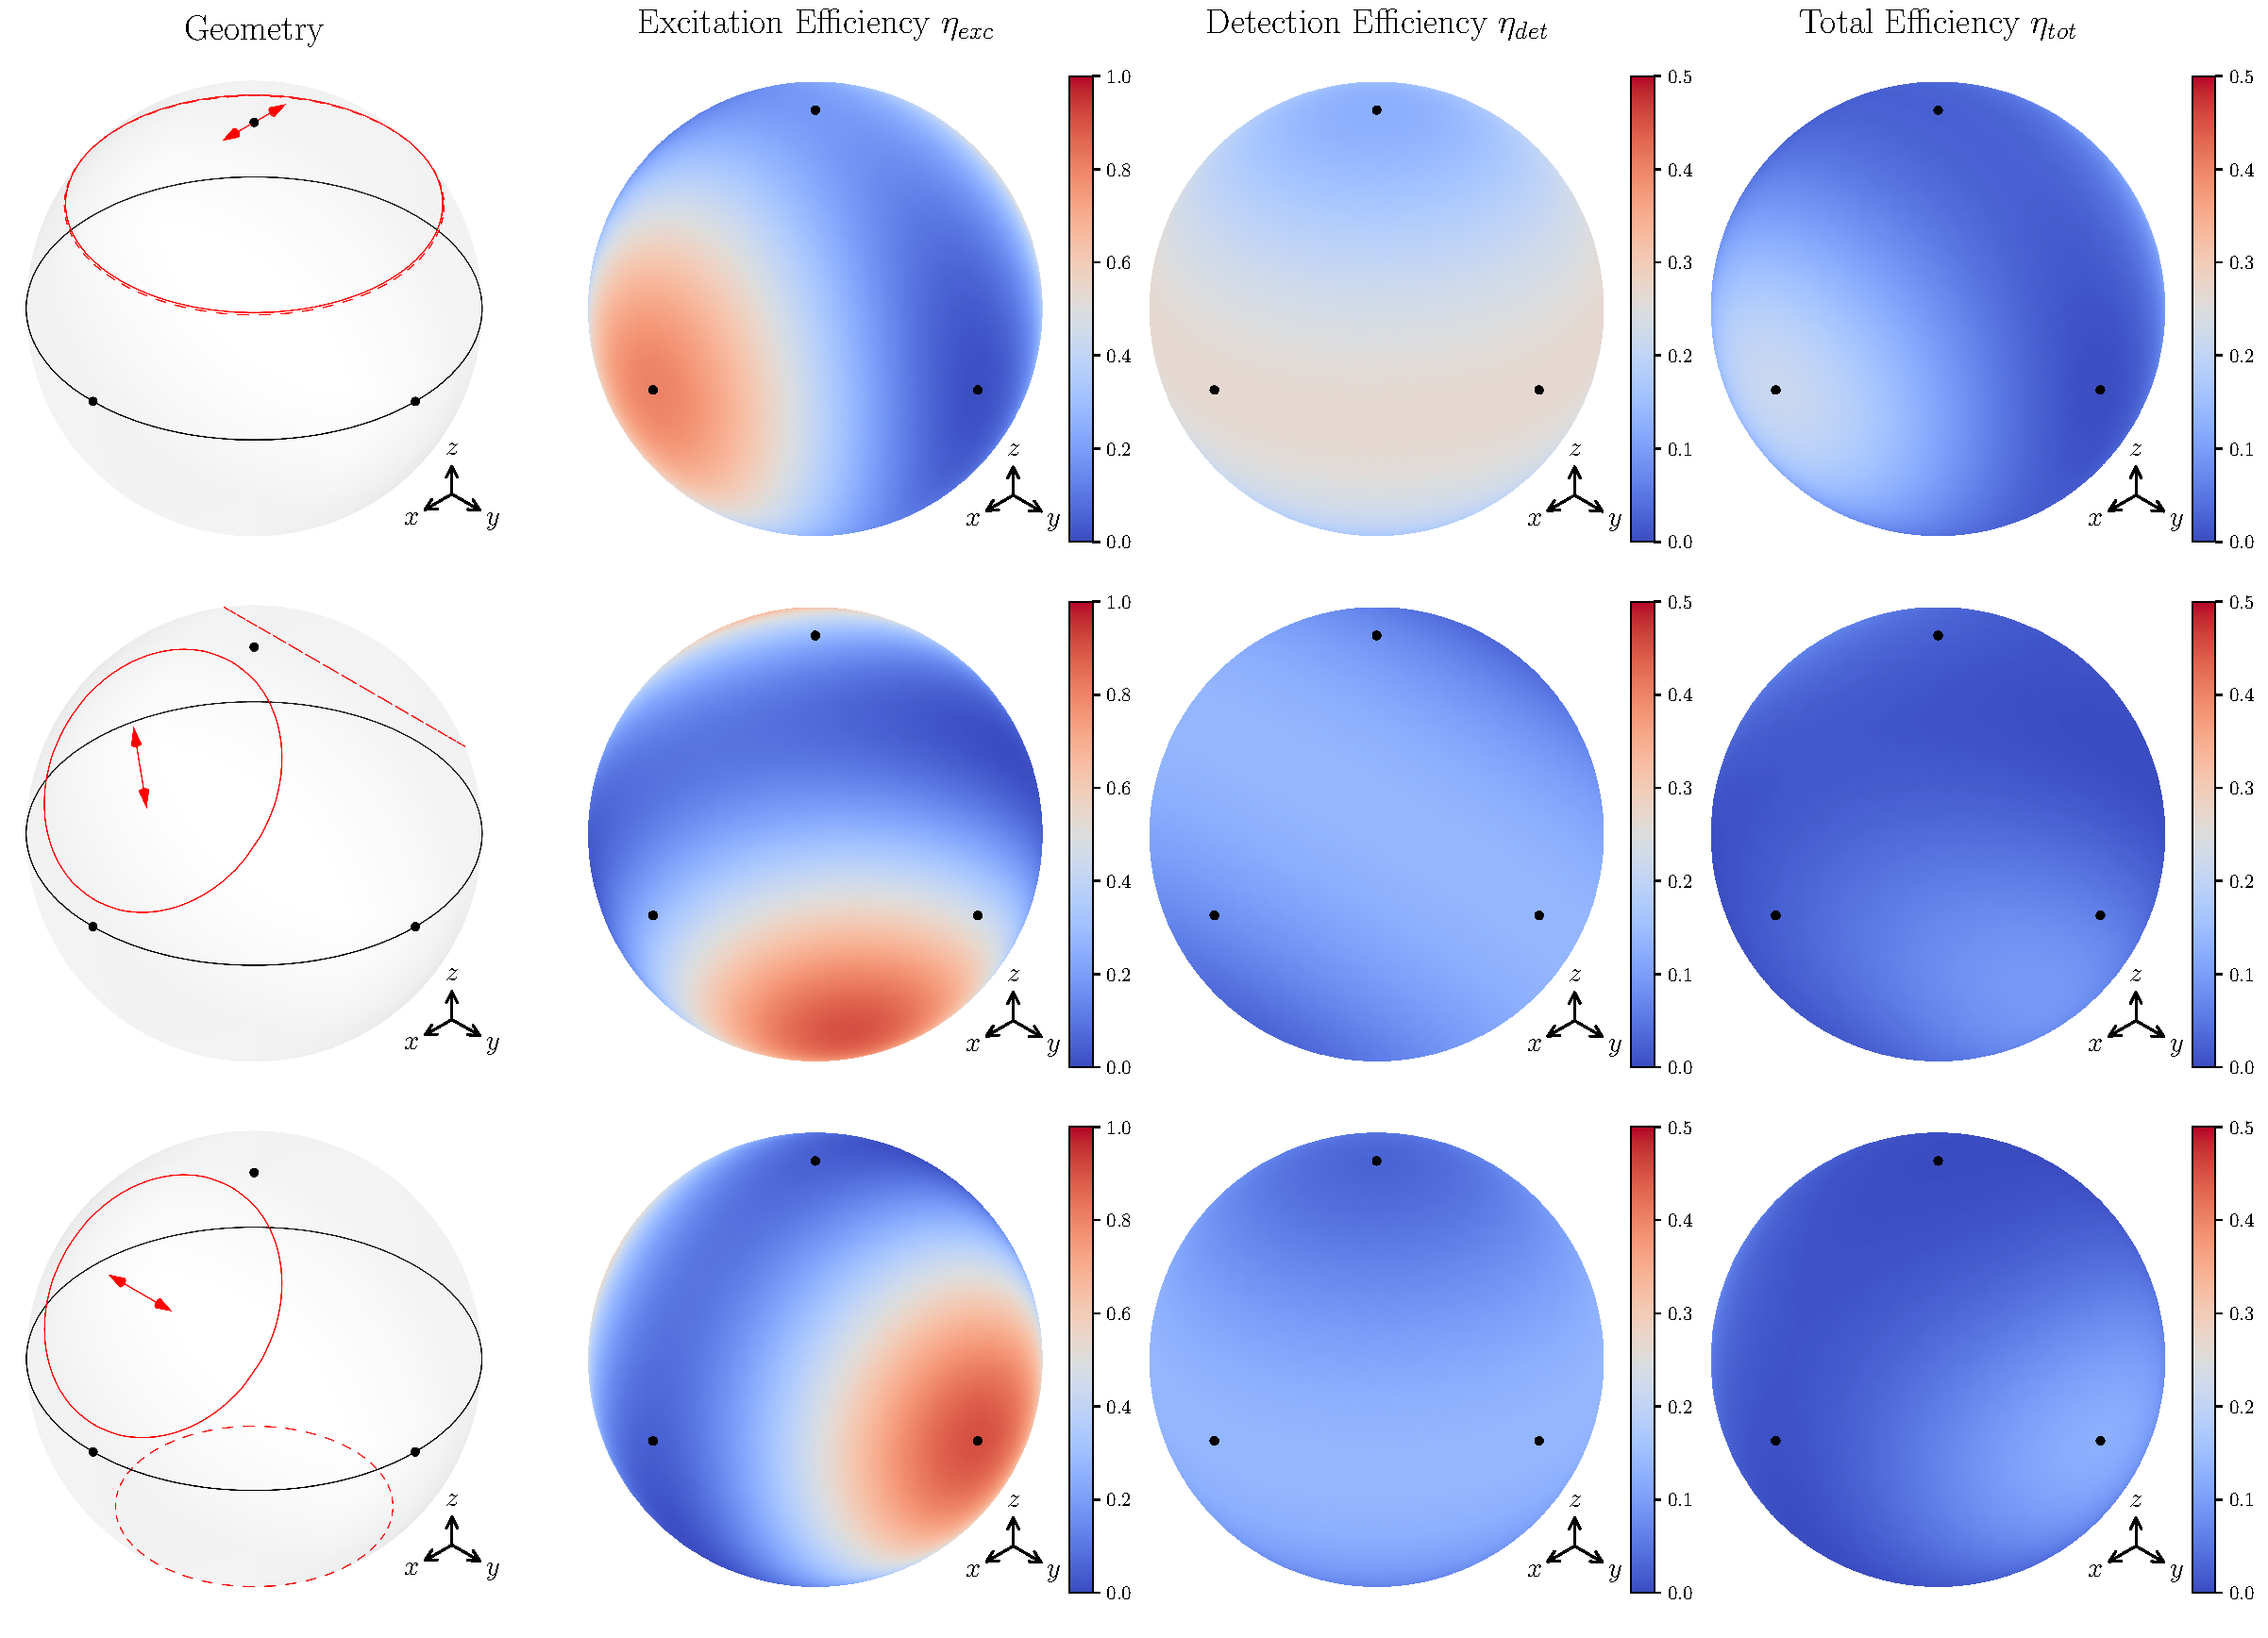
\includegraphics[width=\textwidth]{single-frame}
\caption{Representative examples of the forward model for single frame
  microscopes.\newline \newline \textbf{Columns left to right:} (1) schematics of
  single frame microscopes where the solid line encloses the illumination
  solid angle, the dashed line encloses the detection solid angle, and the arrow
  indicates the transmission axis of the illumination polarizer; (2) the excitation
  efficiency see equation XX; (3) the detection efficiency see equation X; (4)
  the total efficiency see equation X.\newline \newline \textbf{Rows top to
    bottom:} (1) epi-illumination (NA = 1.1) with $x$-polarized light and
  epi-detection (NA = 1.1); (2) orthogonal illumination (NA = 0.8) and detection
  (NA = 0.8); (3) oblique illumination (NA = 0.8) and detection (NA = 0.8).}
\end{figure}

\subsection{Microscope Designs}
Widefield illumination vs light sheet illumination.

- Light sheet has low illumination. 
- Restricted to orthogonal detection. 

\subsection{Evaluation Metrics}
\begin{align}
  F &= \sum_{i=0}^N \frac{1}{I}
  \begin{bmatrix}
    \frac{\partial I}{\partial \Theta}\frac{\partial I}{\partial \Theta}&\frac{\partial I}{\partial \Theta}\frac{\partial I}{\partial \Phi}\\\\
    \frac{\partial I}{\partial \Theta}\frac{\partial I}{\partial \Phi}&\frac{\partial I}{\partial \Phi}\frac{\partial I}{\partial \Phi}\\    
  \end{bmatrix}\\
  \sigma_{\Omega} &= \frac{\sin\Theta}{\sqrt{\text{det}\{F\}}}
\end{align}
We call $\sigma_{\Omega}$ the \emph{solid-angle uncertainty}. 
We sampled $\sigma_{\Omega}$ on 100,000 approximately equally
spaced points on the unit sphere and calculated the \emph{coefficient of variation}
$c_v$ of these points where
\begin{align}
  c_v = \frac{\sigma_{\sigma_{\Omega}}}{\mu_{\sigma_{\Omega}}}
\end{align}

\section{Results}
\subsection{One-Arm Designs}
\begin{figure}[htbp]
\centering\includegraphics[width=\textwidth]{single-arm}
\caption{\textbf{Left:} Schematic of a single-arm four-frame epi-illumination
  microscope with NA = 0.8 and $n = 1.33$.  \textbf{Right:} Solid
  angle uncertainty for the same microscope when $I_{\text{tot}} = 1000$
  photons. Note the regions of high uncertainty near the equator and poles
  as noted in XXX.}
\end{figure}

Can't use $c_v$ because it doesn't converge.

High variance around equator and poles. 

\subsection{Two-Arm Designs}
Widefield vs light sheet.
\begin{figure}[htbp]
\centering\includegraphics[width=\textwidth]{symmetric-widefield}
\caption{}
\end{figure}

\begin{figure}[htbp]
\centering\includegraphics[width=\textwidth]{double-arm}
\caption{}
\end{figure}


\begin{figure}[htbp]
\centering\includegraphics[width=\textwidth]{asymmetric-double}
\caption{}
\end{figure}


Widefield NA vs angle/.

Sweep asymmetry for full NA light sheet.



\subsection{Three-Arm Designs}
\begin{figure}[htbp]
\centering\includegraphics[width=\textwidth]{triple-arm}
\caption{}
\end{figure}

\section{Discussion}

\section{Conclusion}

\section*{Funding}
TODO

\section*{Acknowledgments}
We thank Hari Shroff and Sean Rose for helpful conversations. 

\section*{Disclosures}
The authors declare that there are no conflicts of interest related to this article.

\end{document}
